\appendix

\section{Element Types within LISA}
Here are shown the the visual specifications LISA provides for the ordering and layout of nodes for defining each type of element supported. Each of these types can be classified using the 




\begin{figure}[!h]
\centering
\begin{subfigure}{.5\textwidth}
  \centering
  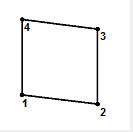
\includegraphics[width=0.3\linewidth]{../Graphics/LISA-quad4.png}
  \caption{quad4 element}
  \label{fig:sub1}
\end{subfigure}%
\begin{subfigure}{.5\textwidth}
  \centering
  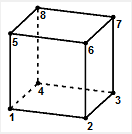
\includegraphics[width=0.3\linewidth]{../Graphics/LISA-hex8.png}
  \caption{hex8 element}
  \label{fig:sub2}
\end{subfigure}
\label{fig:test}
\caption{Square based elements}
\end{figure}


\begin{figure}[!h]
\centering
\begin{subfigure}{.5\textwidth}
  \centering
  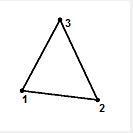
\includegraphics[width=0.3\linewidth]{../Graphics/LISA-tri3.png}
  \caption{tri3 element}
  \label{fig:sub1}
\end{subfigure}%
\begin{subfigure}{.5\textwidth}
  \centering
  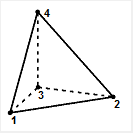
\includegraphics[width=0.3\linewidth]{../Graphics/LISA-tet4.png}
  \caption{tet4 element}
  \label{fig:sub2}
\end{subfigure}
\label{fig:test}
\caption{Triangular based elements}
\end{figure}


\begin{figure}[ht]
\centering
\begin{subfigure}{.5\textwidth}
  \centering
  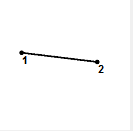
\includegraphics[width=0.3\linewidth]{../Graphics/LISA-line2.png}
  \caption{line2 element}
  \label{fig:sub1}
\end{subfigure}%
\begin{subfigure}{.5\textwidth}
  \centering
  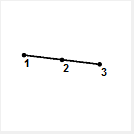
\includegraphics[width=0.3\linewidth]{../Graphics/LISA-line3.png}
  \caption{line3 element}
  \label{fig:sub2}
\end{subfigure}
\label{fig:test}
\caption{Line based elements}
\end{figure} 

%\section{Calculating Centripetal Force For Paper Mill}
%Assuming a constant speed of the paper mill disk at  the following standard calculation was done to compute a forces that could be specified for different elements in order to simulate the effects on the model.

%F = m $\omega^2$ r\\ 

%where: \\ 
%m - mass of object \\ 
%r - radius from centre \\ 
%$\omega$ - angular velocity (radians per second)

%Using the following values for each variable for the plates forming the outside of the paper mill disk the force could be calculated as:

%mass- paper mill is made of steel with each plate having a volume of approximately $24cm^3$ which gives a mass of
%188 grams


\section{Unit Testing}
%Unit tests to validate the correctness of key functionality

\begin{figure}[H]
  \centerline{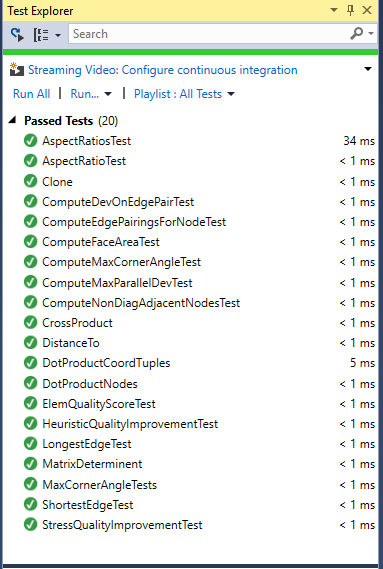
\includegraphics[width=75mm, scale=0.5]{../Graphics/unitTests.png}}
  \caption{Visual Studio window showing the small suite of twenty tests for validating the core functionalyu of the system.}
\end{figure}

%{Centripetal}

\section{Edge Definition Categories}

\textbf{Edge Type}
\begin{itemize}
  \item important long
  \item important
  \item important short
  \item not important
  \item circuit
  \item half circuit
  \item quarter circuit
  \item short for a hole
  \item long for a hole
  \item circuit hole
  \item half circuit hole
  \item quarter circuit hole
\end{itemize}

\textbf{Boundary Type}
\begin{itemize}
  \item free
  \item fixed on one side
  \item fixed on two sides
  \item fixed completely
\end{itemize}

\textbf{Load Type}
\begin{itemize}
  \item no loading
  \item one side loaded
  \item two sides loaded
  \item continuous loading
\end{itemize}

\section{Input and Output Files}
Below can be seen the format of the input files for the system, a LISA .liml and a .json edge definition file\\

\begin{figure}[H]
\centering
\begin{subfigure}{.5\textwidth}
  \centering
  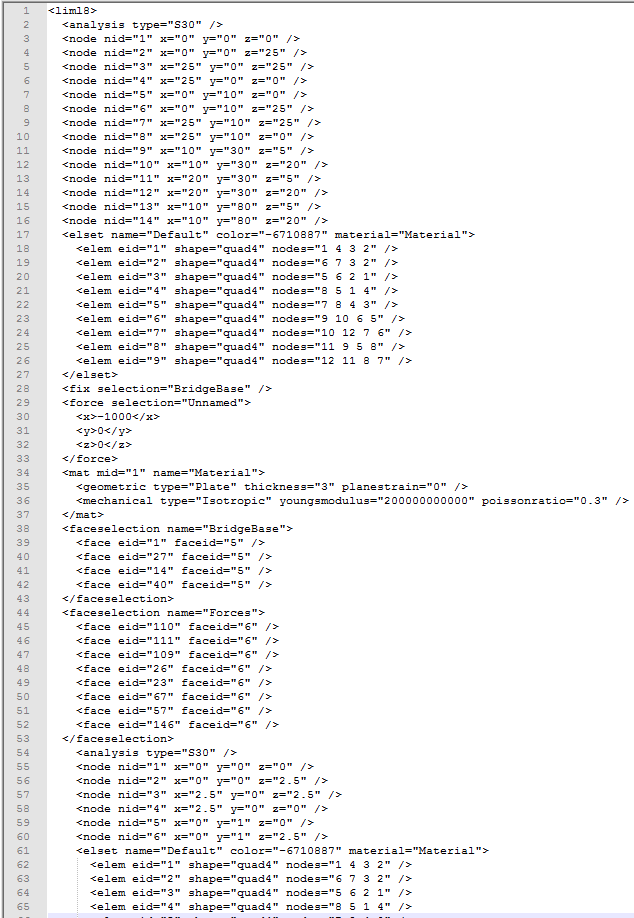
\includegraphics[width=0.6\linewidth]{../Graphics/limlFileLayout.png}
  \caption{Cut down .liml file to show general content which largely defined the schema for the systems data model}
  \label{fig:sub1}
\end{subfigure}%
\begin{subfigure}{.5\textwidth}
  \centering
  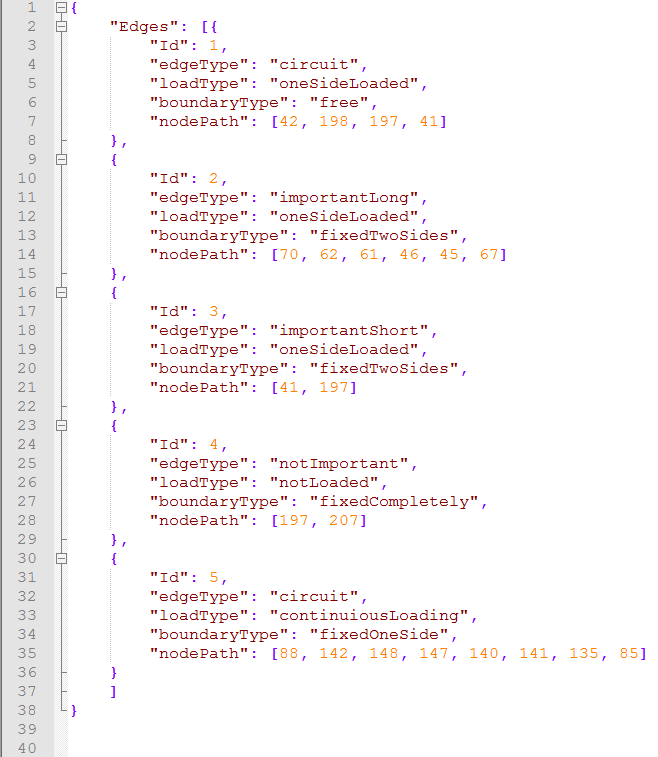
\includegraphics[width=0.8\linewidth]{../Graphics/jsonEdgeFileLayout.png}
  \caption{A json file containing the edges of interest specified by an engineer, this is parsed and the rules are applied to determine the models meshing based on the input}
  \label{fig:sub2}
\end{subfigure}
\label{fig:test}
\end{figure}


\section{Project Layout in Solution Explorer}
Below show the Visual Studio Solution Explorer which provides a general idea of the layout of the project with namespace hierarchies from within an IDE.

\begin{figure}[H]
  \centerline{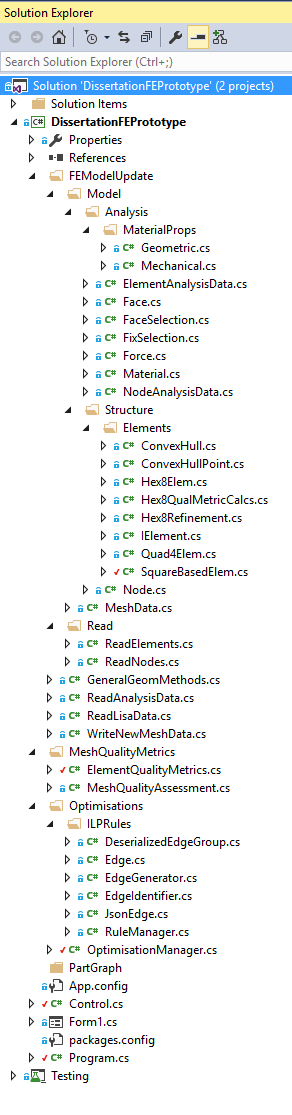
\includegraphics[width=60mm, height=180mm, scale=0.25]{../Graphics/VSolutionExplorer.png}}
  \caption{The metrics calculated by visual studio for all high level modules in the system}
\end{figure}




\section{Doxygen Documentation}
\begin{figure}[H]
  \centerline{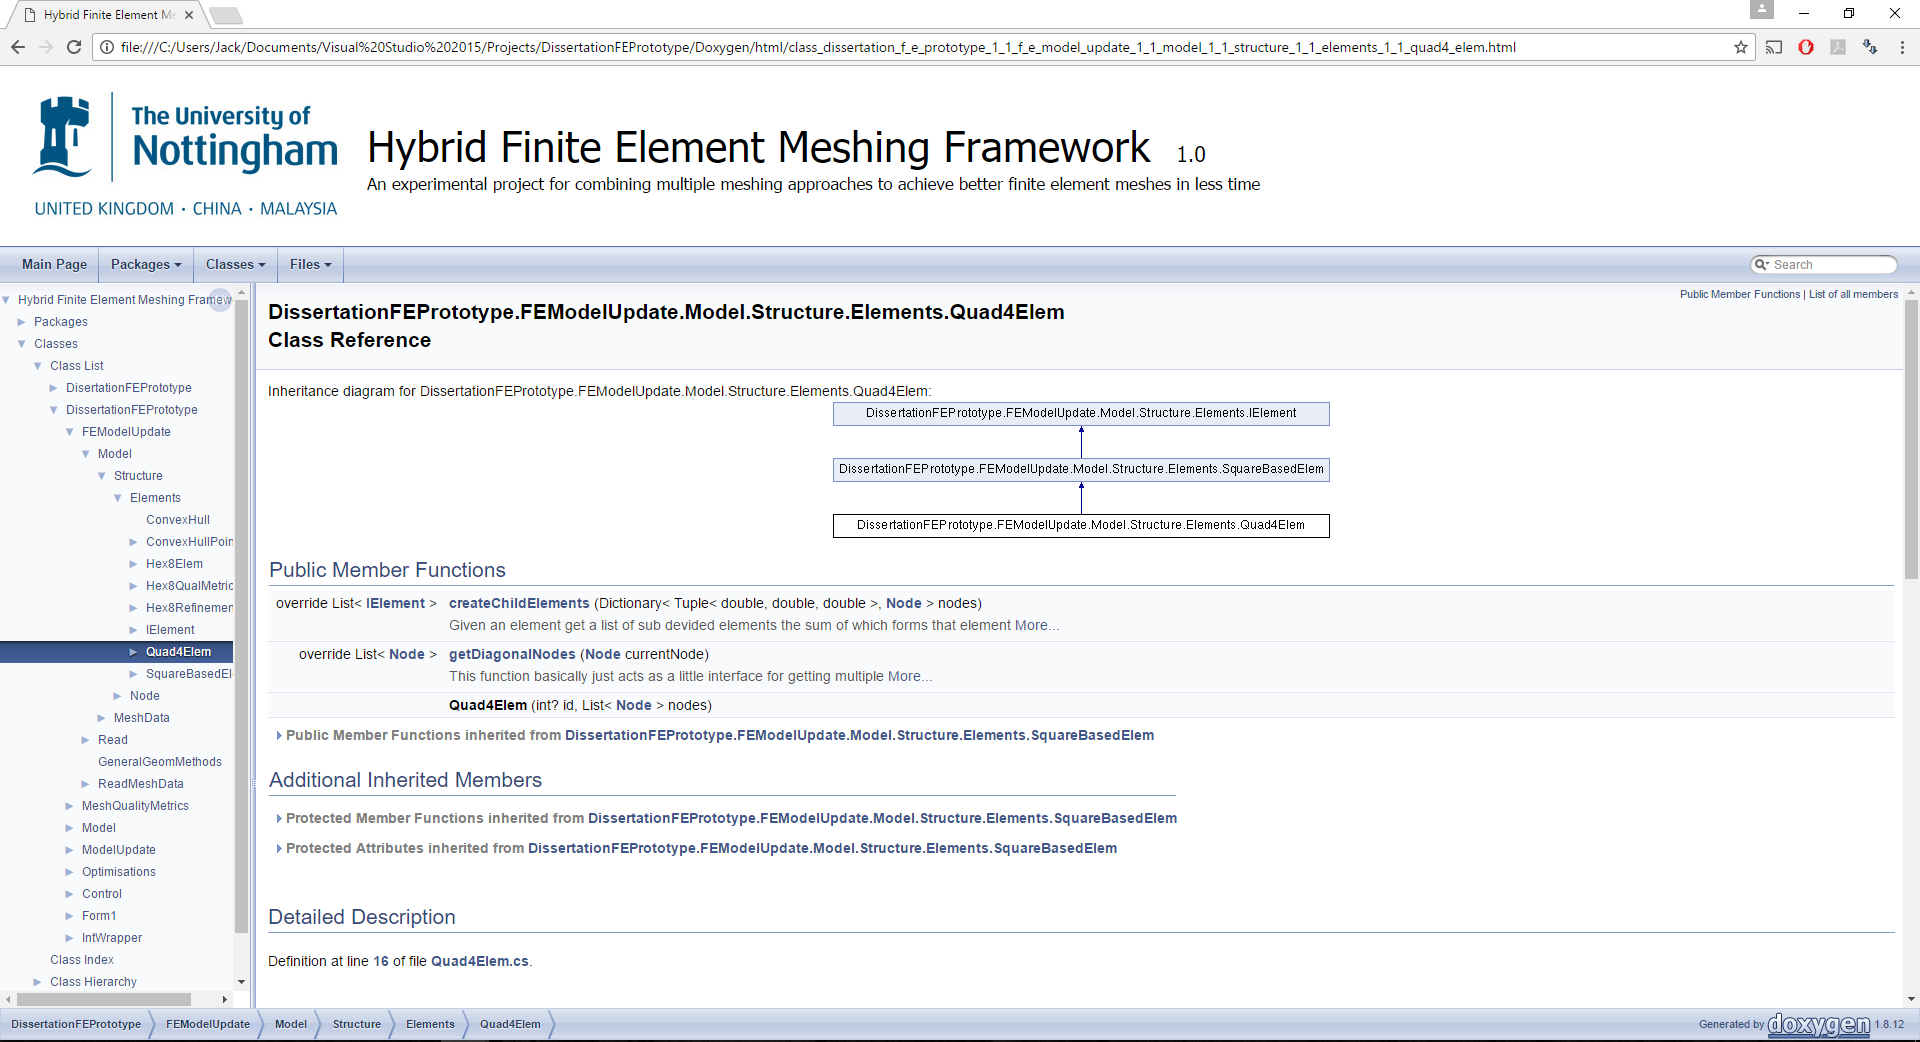
\includegraphics[width=165mm,  scale=0.5]{../Graphics/Doxygen/Quad4Element.png}}
  \caption{The manual page for the Quad4 element class with the class hierarchy and specific public methods}
\end{figure}

\begin{figure}[H]
  \centerline{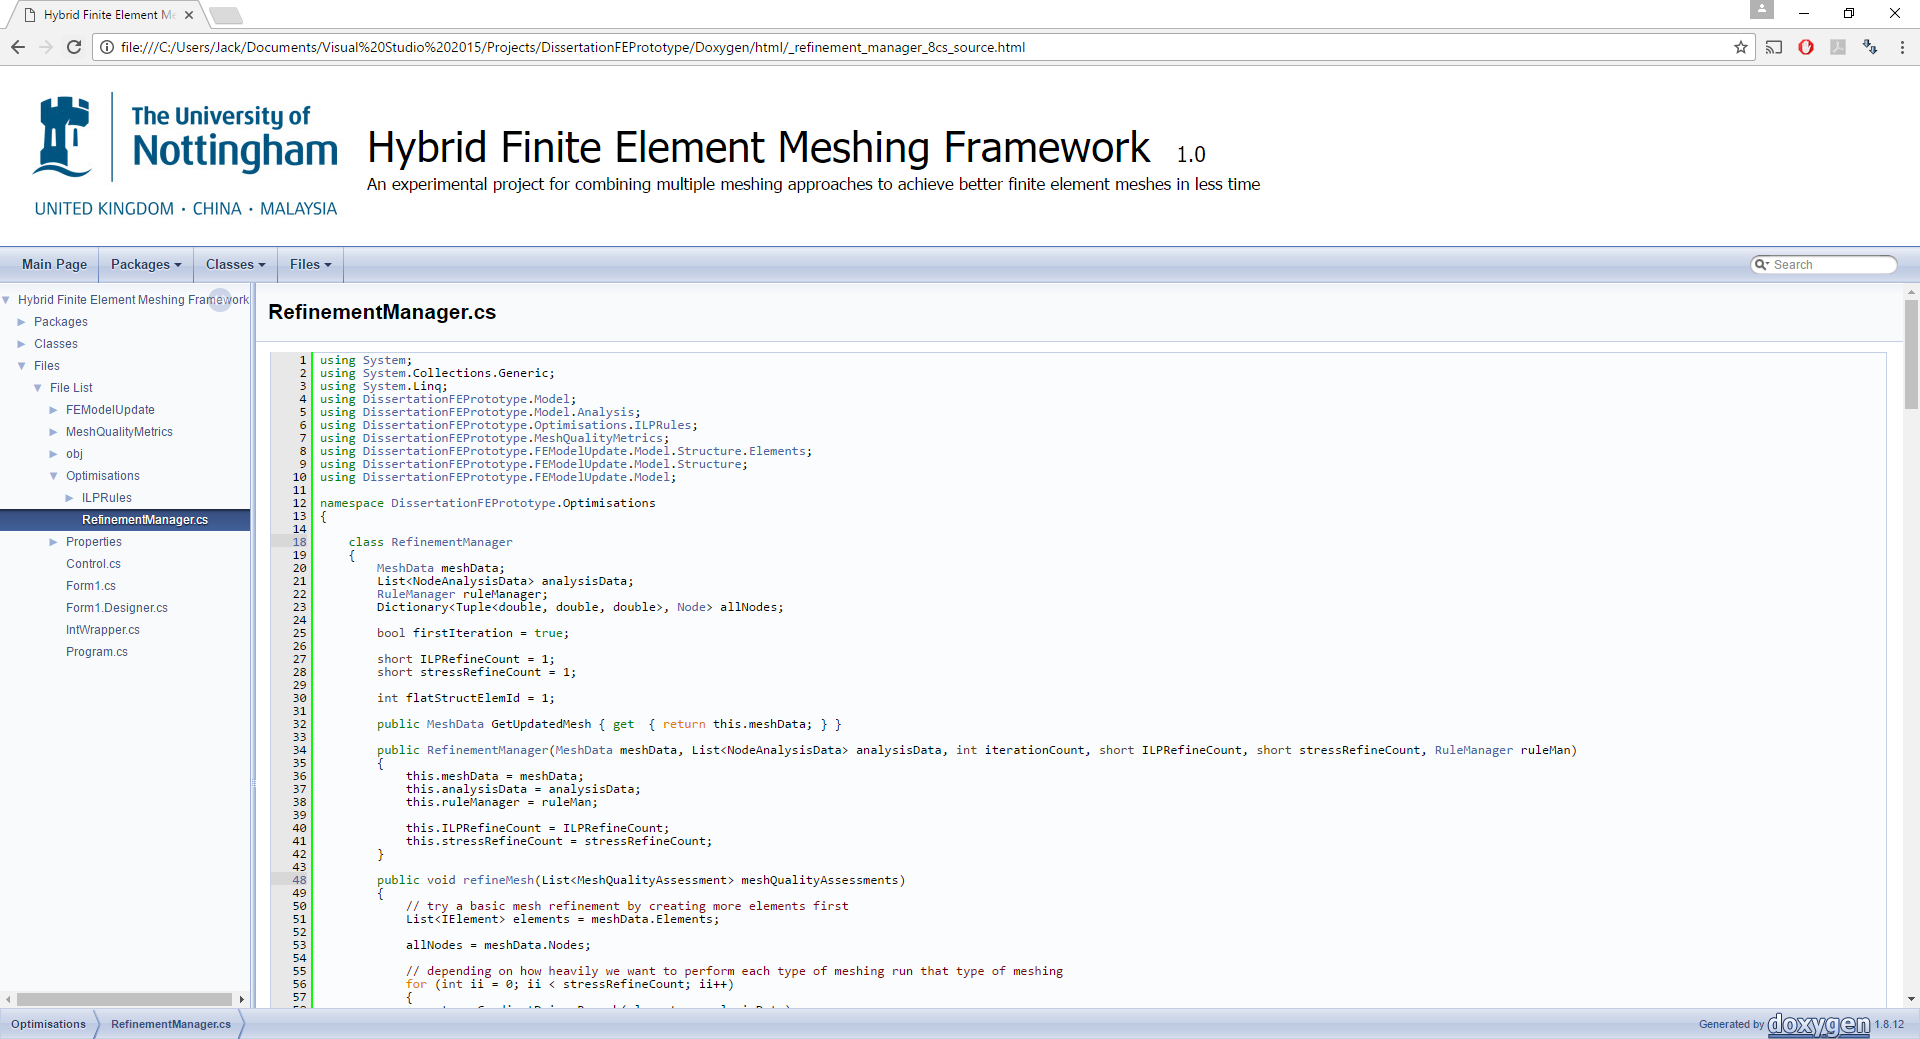
\includegraphics[width=165mm,  scale=0.5]{../Graphics/Doxygen/RefinementManager.png}}
  \caption{Code for the RefinementManager class viewed within the Doxygen UI}
\end{figure}



\section{Software Quality Metrics}
\begin{figure}[H]
  \centerline{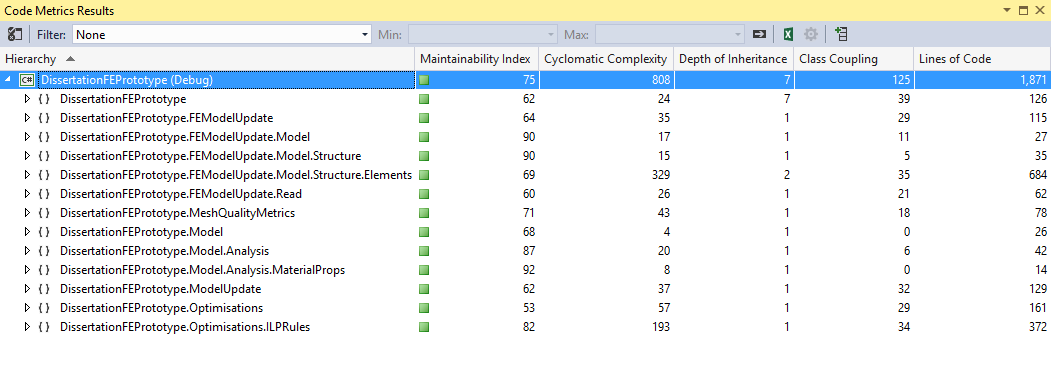
\includegraphics[width=165mm, scale=0.5]{../Graphics/softwareQualityMetrics.png}}
  \caption{The metrics calculated by visual studio for all high level modules in the system}
\end{figure}

\begin{figure}[H]
  \centerline{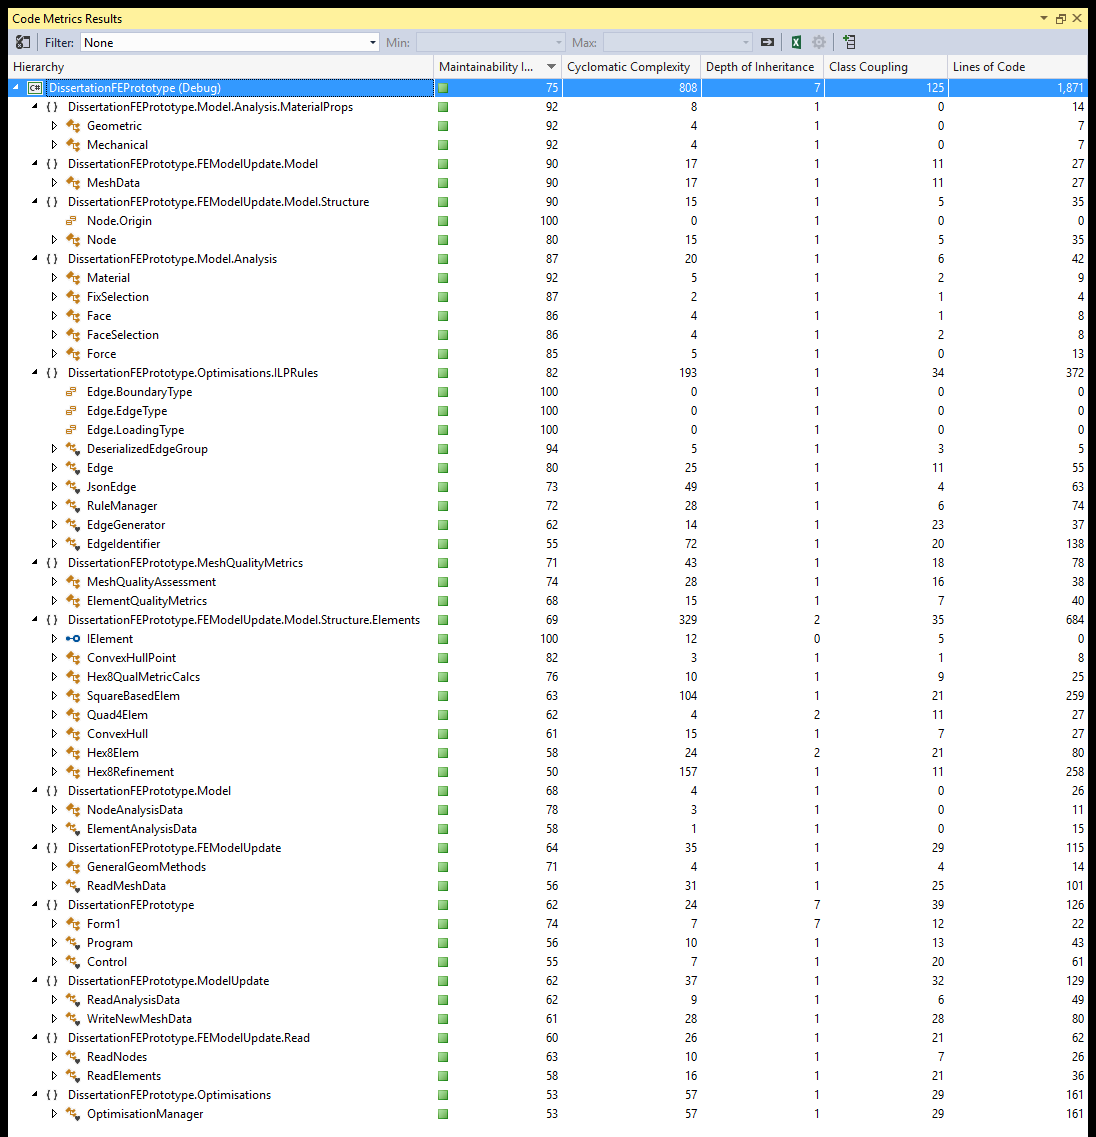
\includegraphics[width=165mm, scale=0.5]{../Graphics/qualityMetricsExpanded.png}}
  \caption{The metrics calculated by visual studio for the all classes in the final system}
\end{figure}


\section{Mesh Refinements}
This appendix item attempt too show the general mesh that are formed using the heuristic and stress based refinement strategy with examples of where a heuristic has been placed well and poorly and where there is also variation in the threshold used to decide whether elements are meshed with the stress variable. Although in the rest of the models we are looking for stress since this is the primary variable of interest displacement has been selected as the analysis variable for displacement due to it producing a clearer gradient than stress.


\subsection{Heuristic Refinement}



\begin{figure}[H]
\centering
\begin{subfigure}{.5\textwidth}
  \centering
	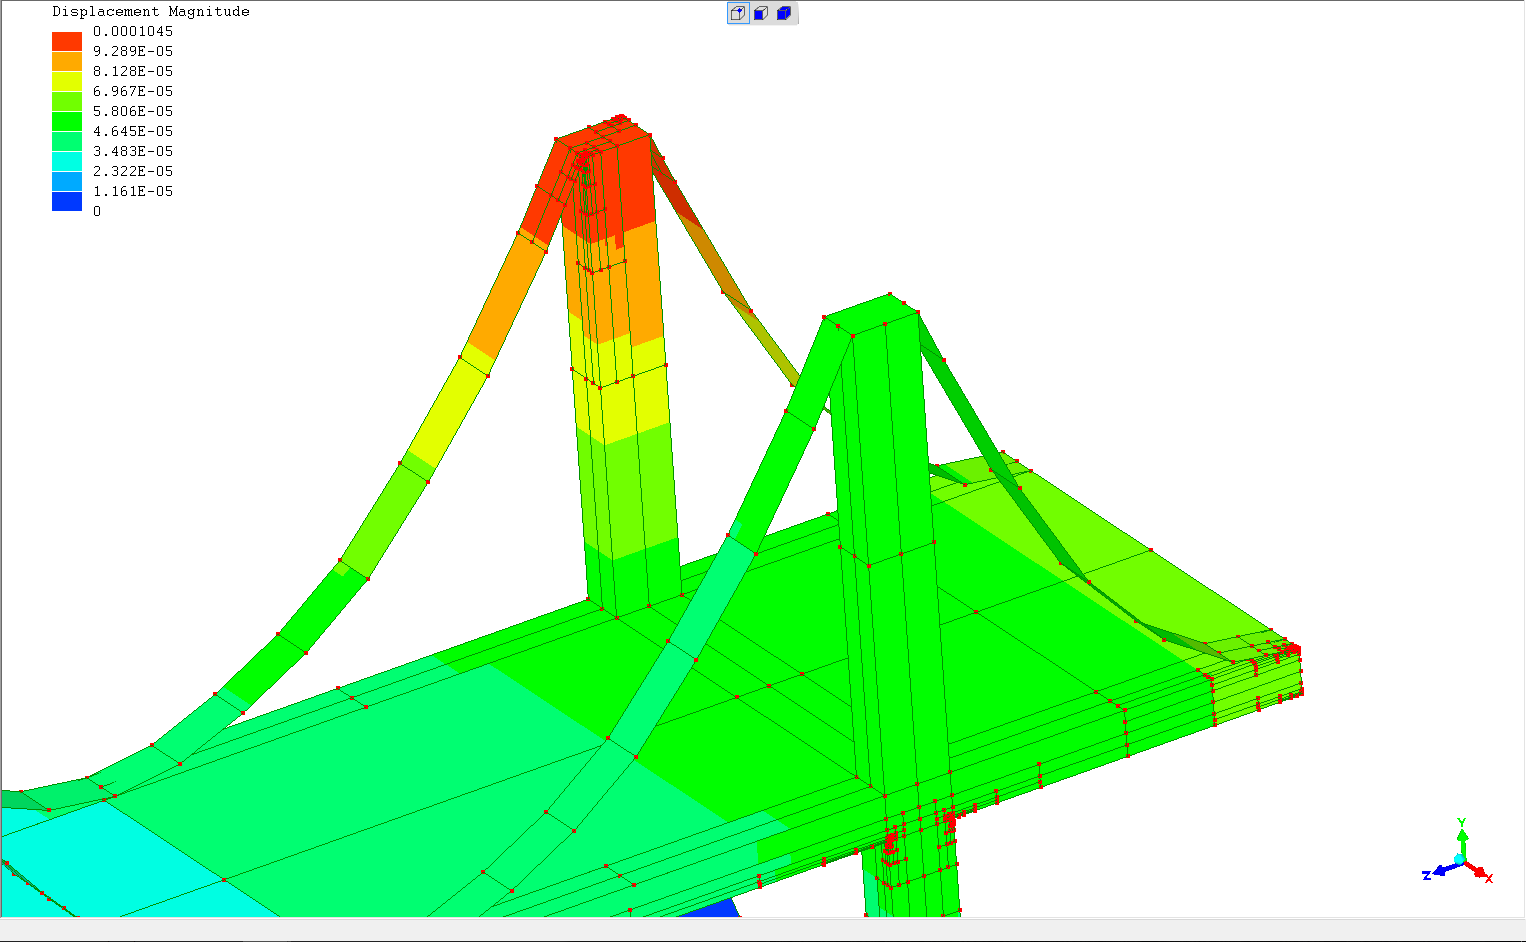
\includegraphics[width=80mm, scale=0.5]{../Graphics/BridgeCrossLoading/bestEdgeSpecResults.png}
  \caption{Important edges specified effectively to facilitate preemptive meshing of area which undergoes high stress}
  \label{fig:sub1}
\end{subfigure}%
\begin{subfigure}{.5\textwidth}
  \centering
  \centerline{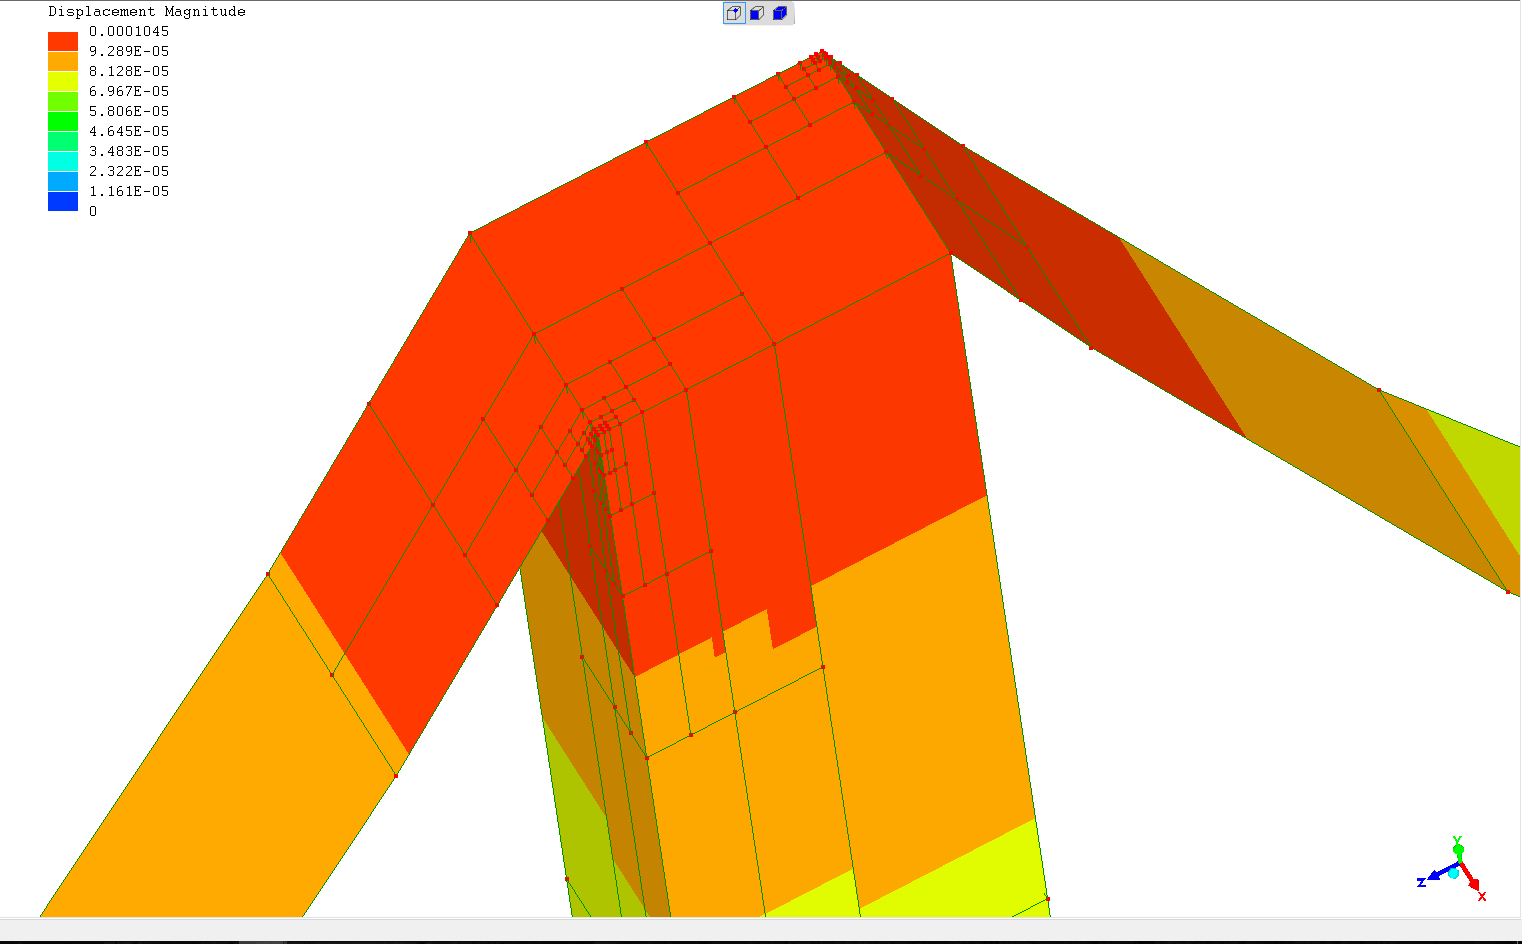
\includegraphics[width=80mm, scale=0.5]{../Graphics/BridgeCrossLoading/bestEdgeSpecResultsCloseUp.png}}
  \caption{Close up view of refinement for high displacement areas }
  \label{fig:sub2}
\end{subfigure}
\label{fig:test}
\end{figure}


\begin{figure}[H]
  \centerline{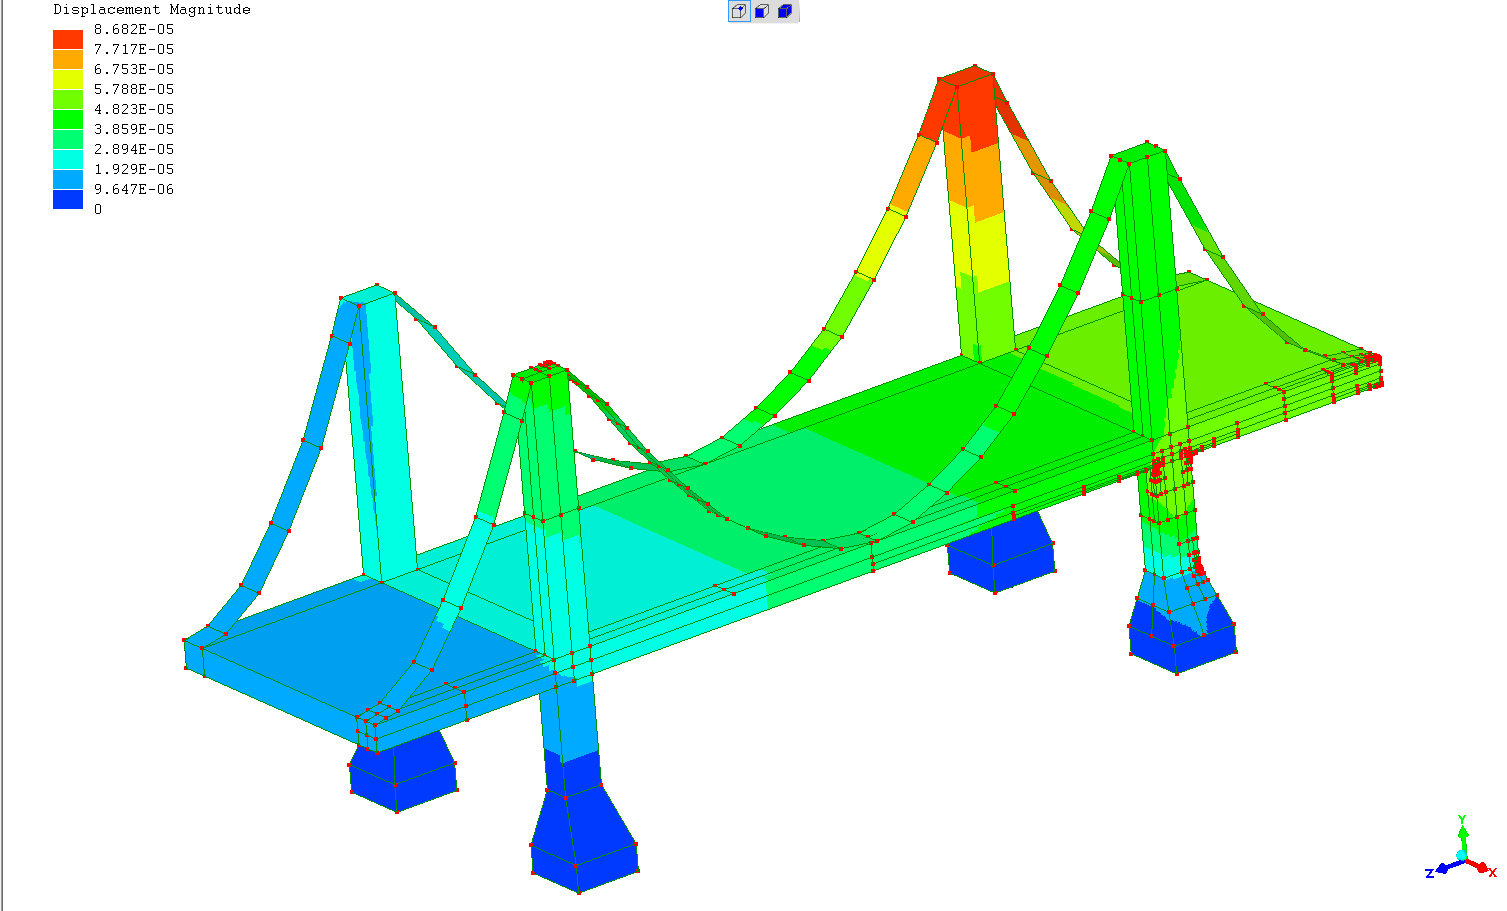
\includegraphics[width=165mm, scale=0.5]{../Graphics/BridgeCrossLoading/okEdgeSpecResults.png}}
  \caption{Important edges more poorly specified missing high displacement region on top of furthest suspension bridge tower}
\end{figure}

\subsection{Stress Refinement}
\begin{figure}[H]
  \centerline{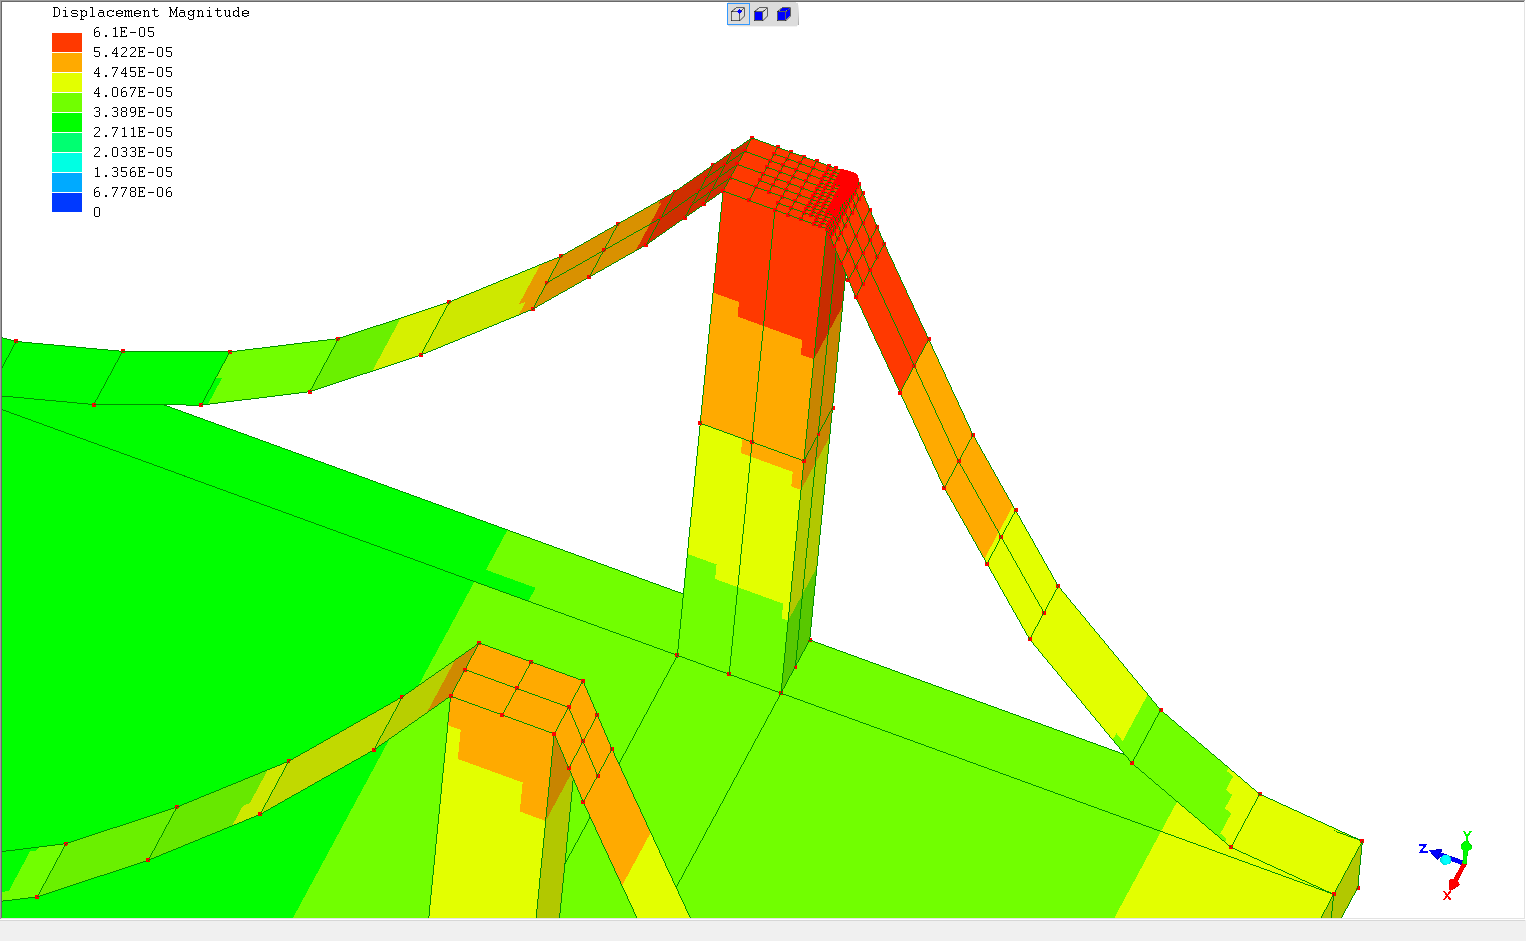
\includegraphics[width=165mm, scale=0.5]{../Graphics/BridgeCrossLoading/the90thPercentileRefinement.png}}
  \caption{Iterative stress/ displacement refinement method used to focus meshing on the top 6\% most displaced region of model}
\end{figure}

\begin{figure}[H]
  \centerline{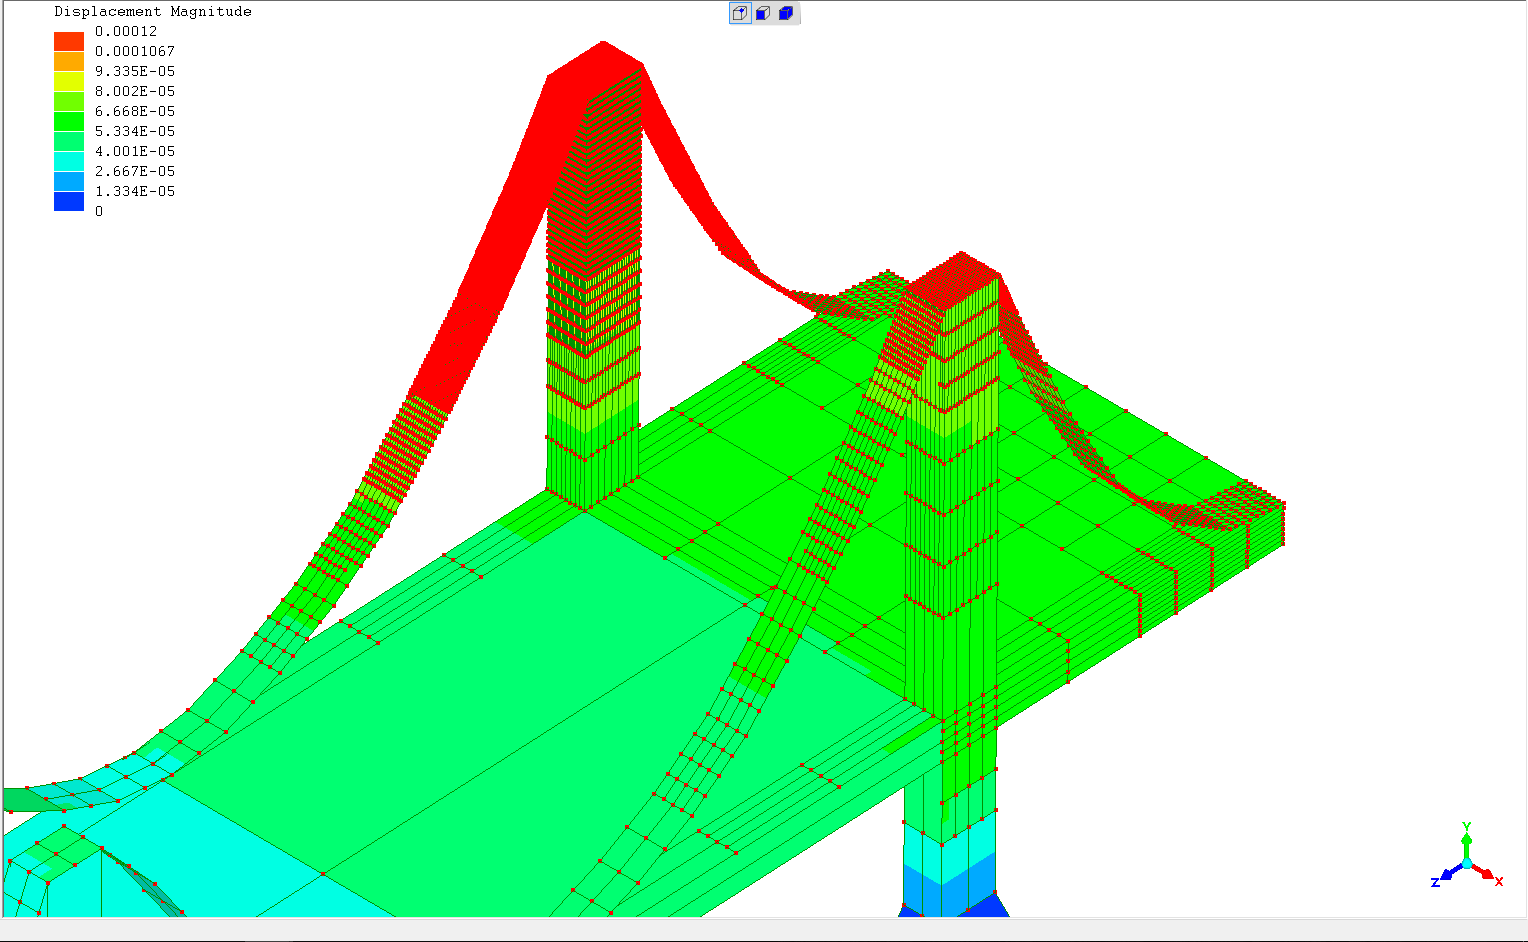
\includegraphics[width=165mm, scale=0.5]{../Graphics/BridgeCrossLoading/aboveAverageRefinement2.png}}
  \caption{Iterative refinement of high displacement but with the remesh threshold specified as the average displacement across the whole model. A consequence of this is the gradient of refinement fidelity that can be seen corresponding to the importance of that part of the structure}
\end{figure}


\begin{figure}[H]
  \centerline{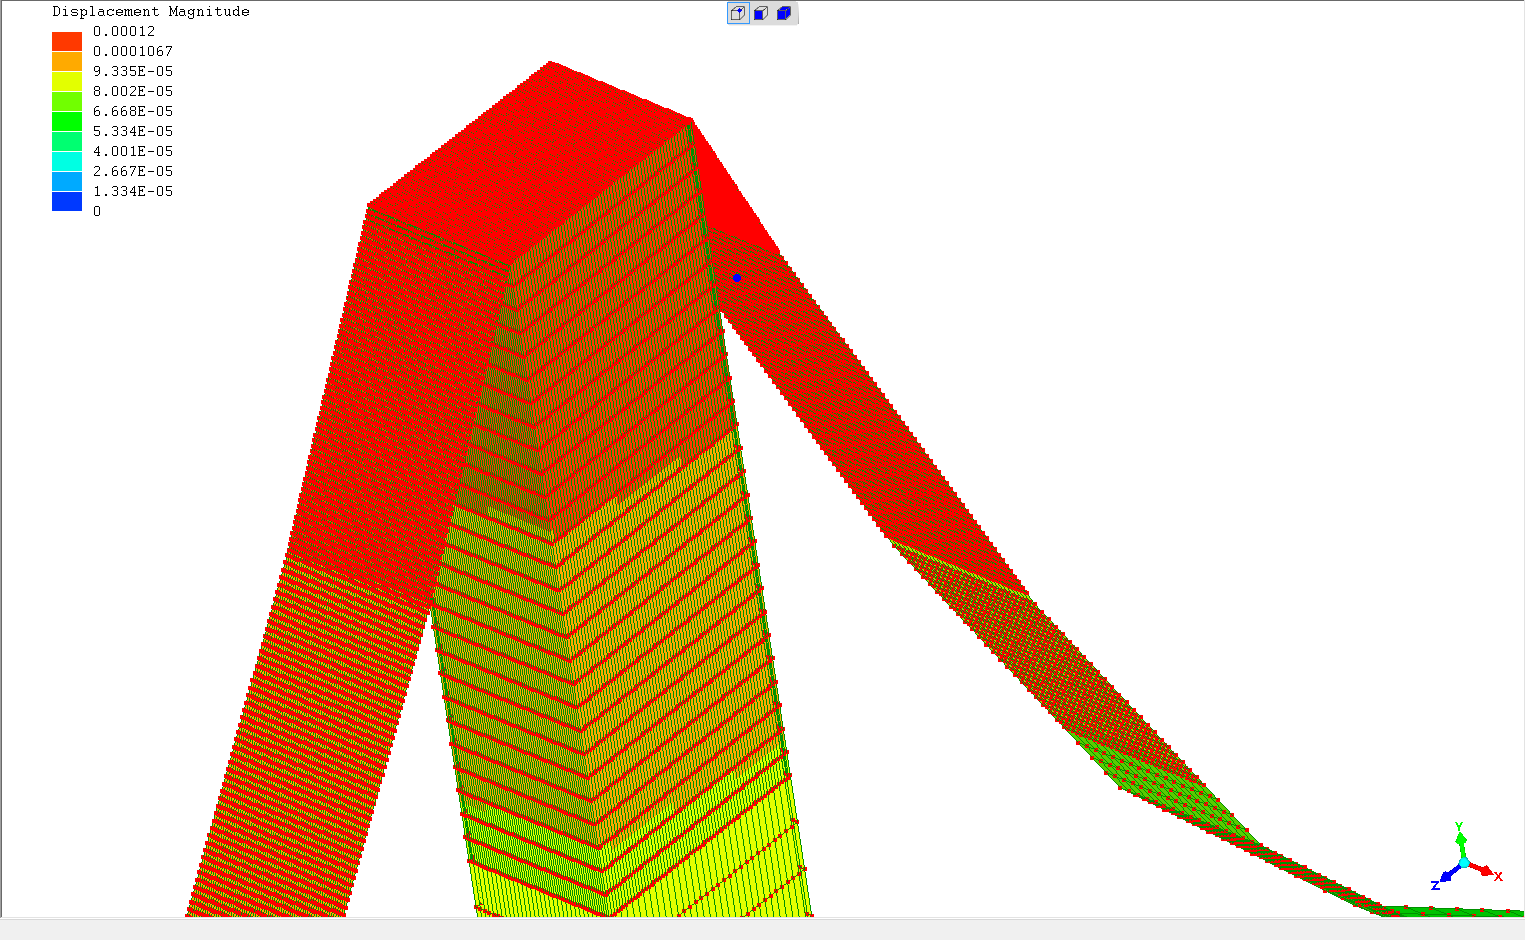
\includegraphics[width=165mm, scale=0.5]{../Graphics/BridgeCrossLoading/aboveAverageRefinement.png}}
  \caption{Closer view of very high meshing intensity}
\end{figure}
%\end{changemargin}



\section{Paper Mill Simulation Results}
For the paper mill simulation angular forces were set up around the outside of the disk so as to simulate the effect of the disk rotating at high speed, with it also being pulled outwards in the axial direction. This generated some interesting patches of stress across the main body of the structure which could easily be specified as edge rules. Looking at figure 34 it is possible to see very high range of stress values for stress observable within the model as a consequence of stress concentrating at particular points.

% edge assignement drawign here

\colorbox{yellow}{Still need to add some more to this bit}

\begin{figure}[H]
\centering
\begin{subfigure}{.5\textwidth}
  \centering
  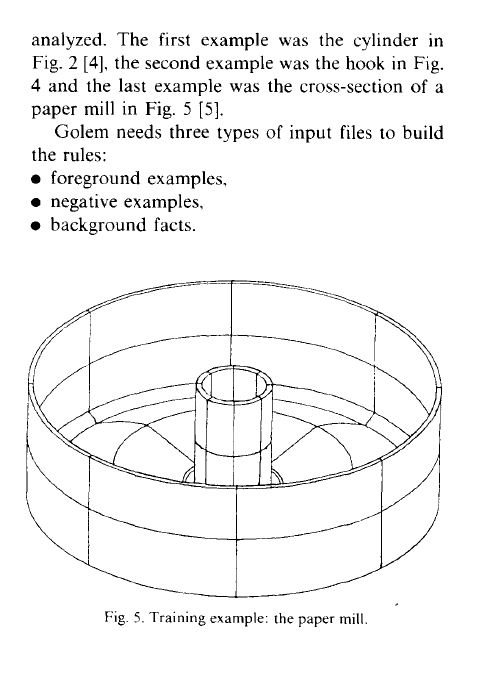
\includegraphics[width=0.9\linewidth]{../Graphics/PaperMillDolsak.jpeg}
  \caption{Half of Cylinder structure described by dolsak in his papers for training ILP system}
  \label{fig:sub1}
\end{subfigure}%
\begin{subfigure}{.5\textwidth}
  \centering
  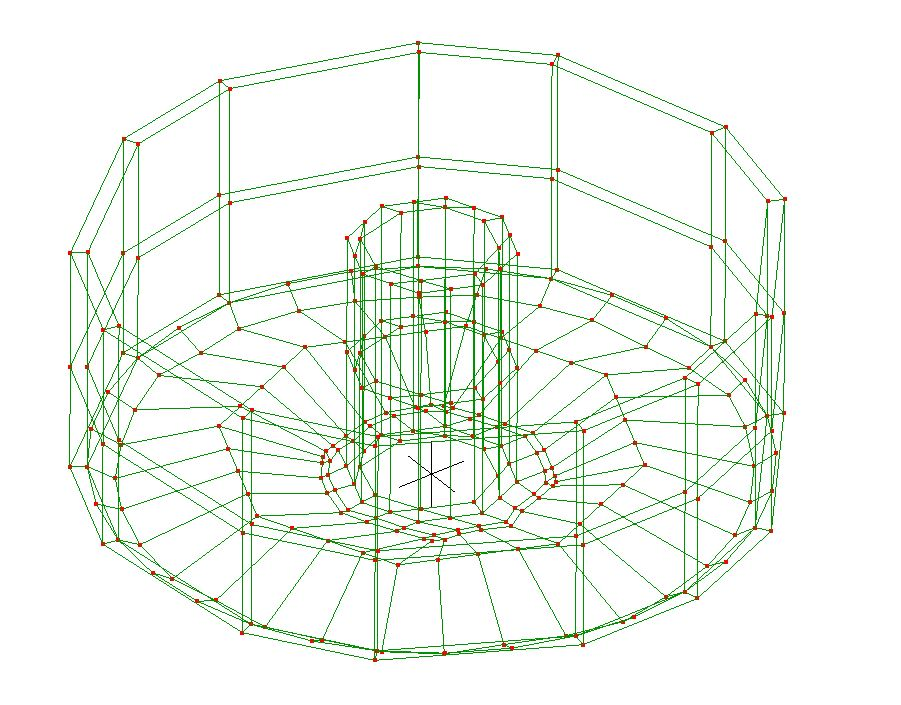
\includegraphics[width=0.9\linewidth]{../Graphics/PaperMillWithinLisa.jpeg}
  \caption{Replication of mesh structure specified by Dolsak within his paper \cite{Dolsak91}}
  \label{fig:sub2}
\end{subfigure}
\label{fig:test}
  \caption{Execution time increase compared to the amount of information revealed for the different approaches}
 \end{figure}
 
 \begin{figure}[H]
  \centerline{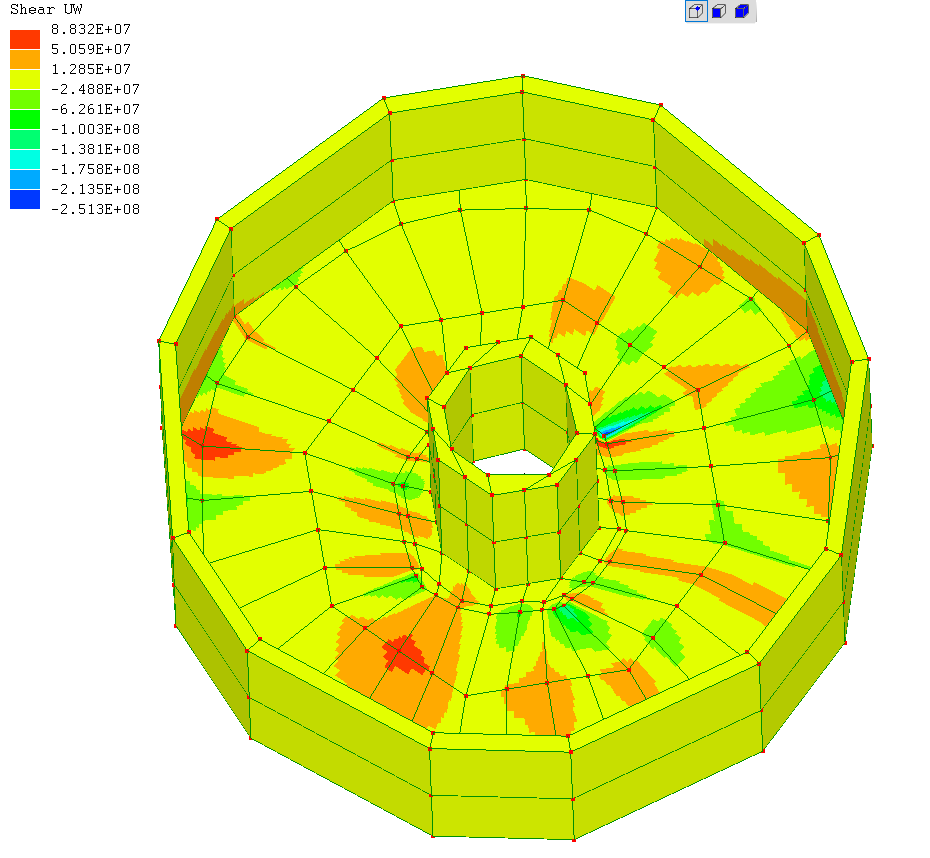
\includegraphics[width=120mm, scale=0.5]{../Graphics/PaperMillStress/PaperMillFirstUWMesh.png}}
  \caption{The initially stressed paper mill part used to define edge sets for further meshing, stress concentrations can be observed in red with colour coding at the top indicating showing a rapidly exponential increase concentrated at those points}
\end{figure}


\begin{figure}[H]
  \centerline{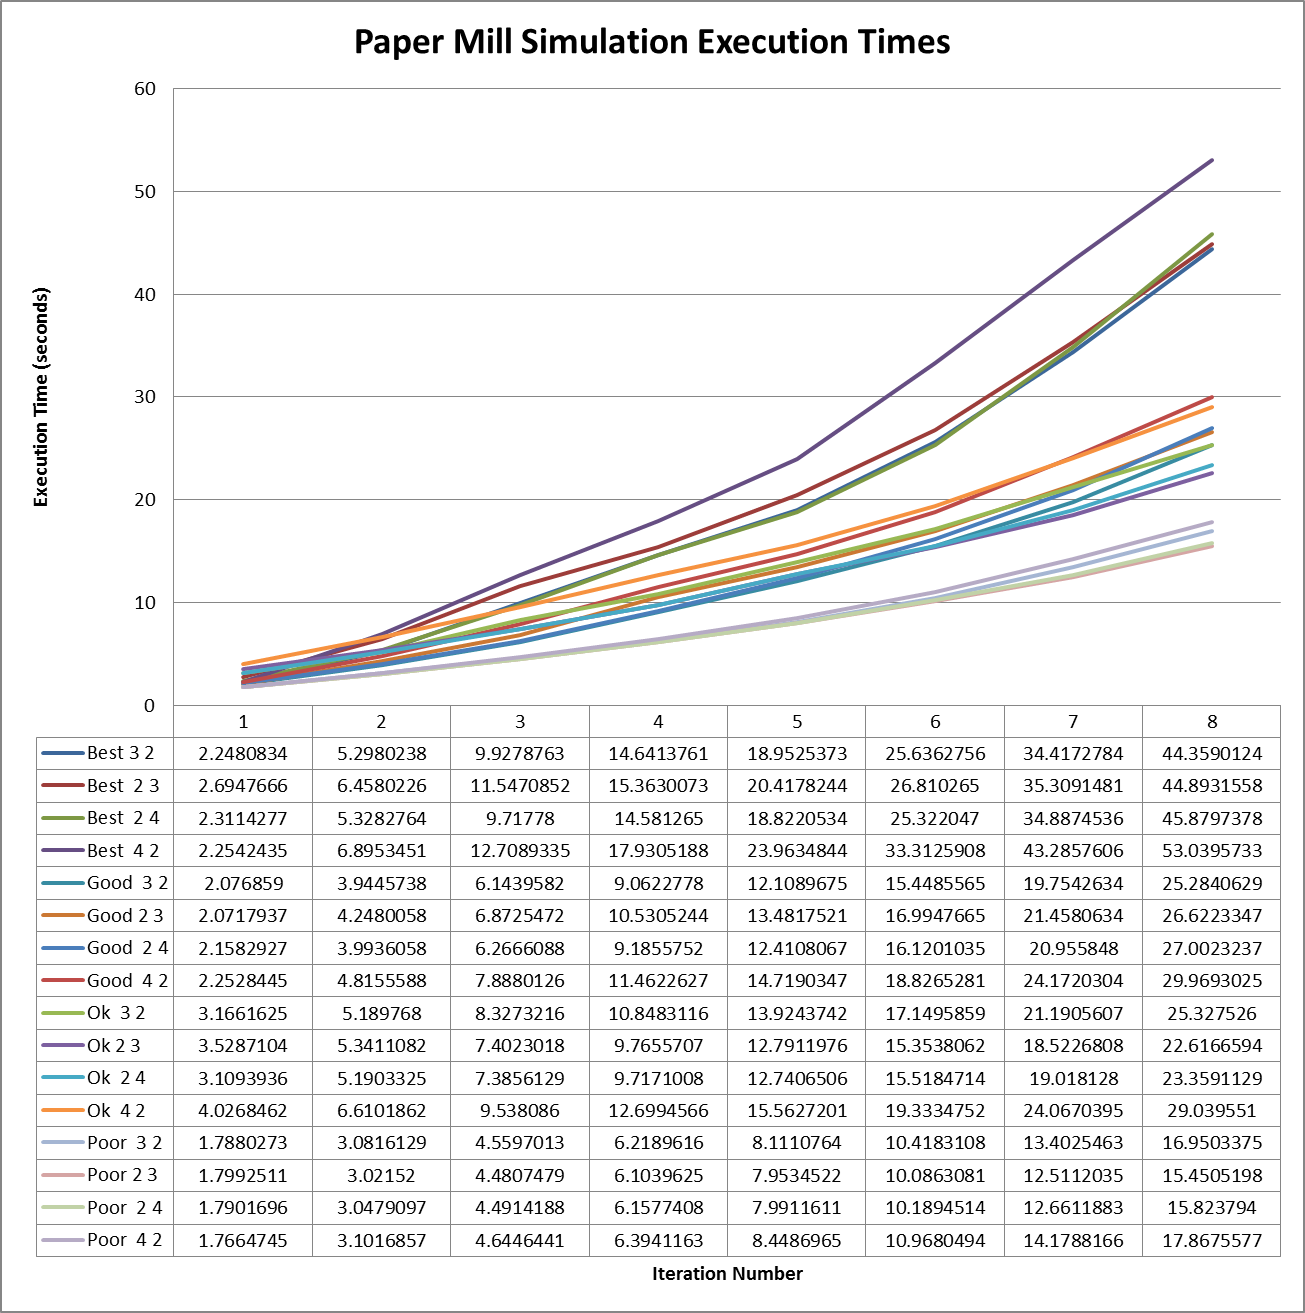
\includegraphics[width=120mm, scale=0.5]{../Graphics/Graphs/PaperMillExecutionTimes.png}}
  \caption{Time taken per iteration using the different hybrid weightings with varying edge quality specifications}
\end{figure}

 \begin{figure}[H]
  \centerline{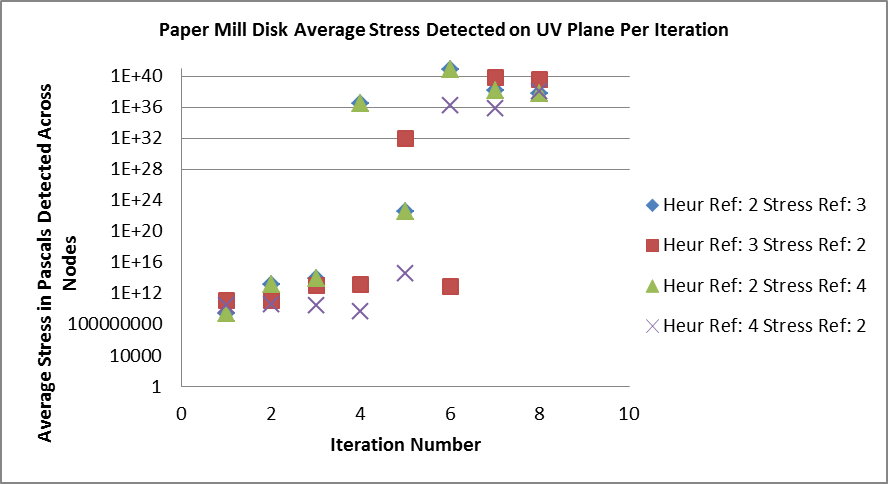
\includegraphics[width=120mm, scale=0.5]{../Graphics/Graphs/PaperMillAverageStressRevealed.png}}
  \caption{Improvement in average stress detected across all nodes within the model over multiple iterations, results for each weighting with different edge heuristics also averaged}
\end{figure}


\section{Half Cylinder Simulation Results}
The half cylinder was the third model used to test the system. 




\begin{figure}[H]
\centering
\begin{subfigure}{.5\textwidth}
  \centering
  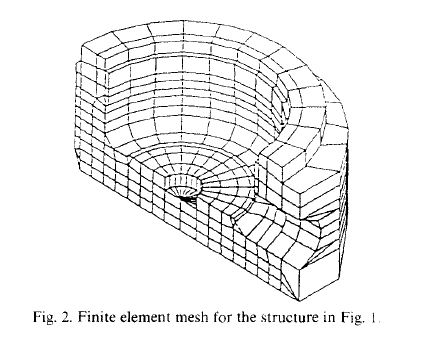
\includegraphics[width=0.9\linewidth]{../Graphics/HalfCylinder/DolsakCylinderMeshed.jpeg}
  \caption{Half of Cylinder structure described by dolsak in his papers for training ILP system}
  \label{fig:sub1}
\end{subfigure}%
\begin{subfigure}{.5\textwidth}
  \centering
  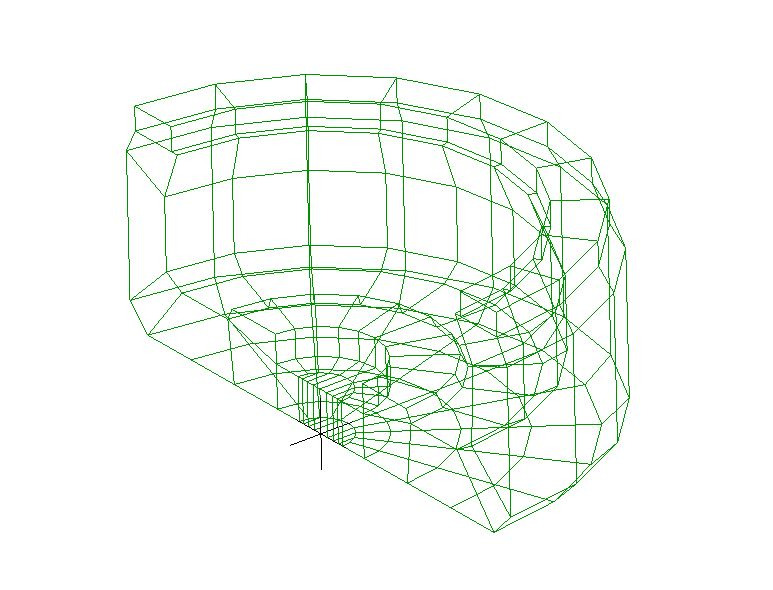
\includegraphics[width=0.9\linewidth]{../Graphics/HalfCylinder/DolsakCylinderWithinLisa.jpeg}
  \caption{Replication of mesh structure specified by Dolsak within his paper \cite{Dolsak91}}
  \label{fig:sub2}
\end{subfigure}
\label{fig:test}
  \caption{Execution time increase compared to the amount of information revealed for the different approaches}
 \end{figure}
 
 
 \begin{figure}[H]
\centering
\begin{subfigure}{.5\textwidth}
  \centering
  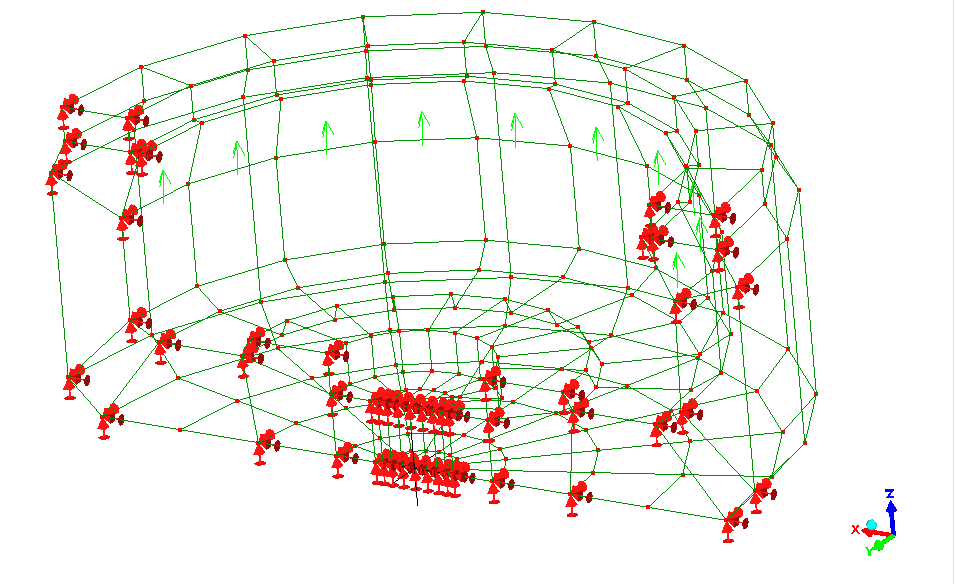
\includegraphics[width=0.9\linewidth]{../Graphics/HalfCylinder/ForcesAndConstraintsOnCylinderPNG.png}
  \caption{Cylinder Constrained by its adjacent half with forces applied up and outwards on its inner rim}
  \label{fig:sub1}
\end{subfigure}%
\begin{subfigure}{.5\textwidth}
  \centering
  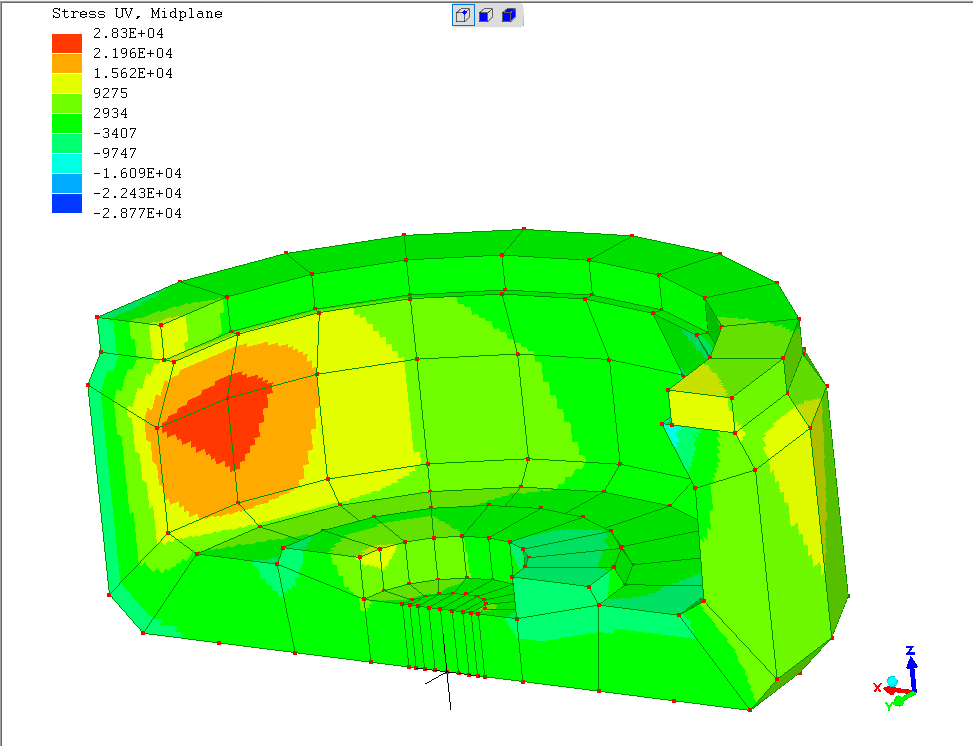
\includegraphics[width=0.9\linewidth]{../Graphics/HalfCylinder/InitialStress.png}
  \caption{Half cylinder with an initial stress concentration having performed a simple execution of the model.}
  \label{fig:sub2}
\end{subfigure}
\label{fig:test}
  \caption{Initial configuration for the half cylinder and some stresses revealed on the structure}
 \end{figure}
 
\begin{figure}[H]
  \centerline{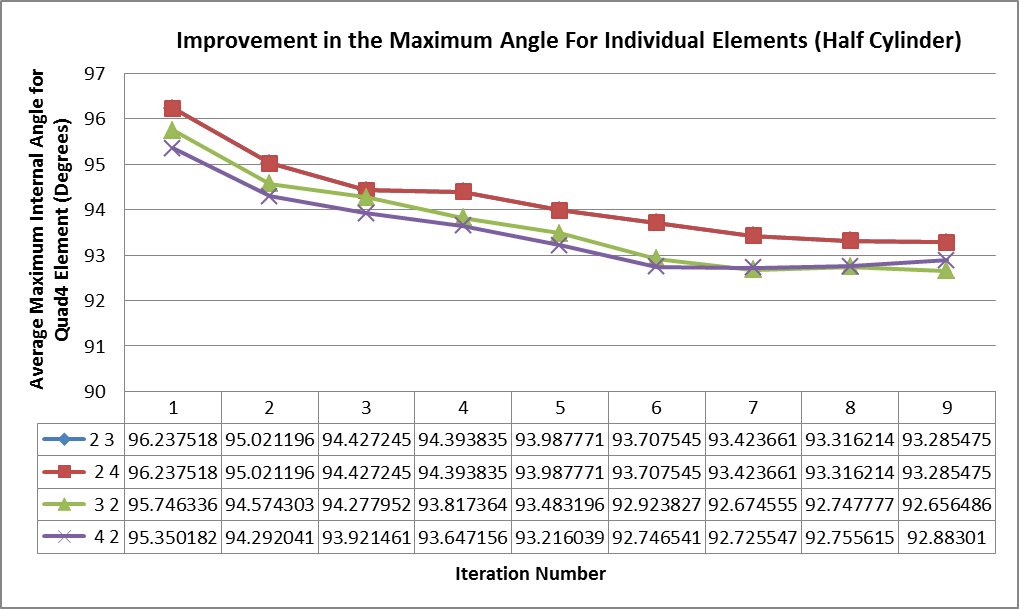
\includegraphics[width=120mm, scale=0.5]{../Graphics/HalfCylinder/ImprovementInMaxCornerAngles.png}}
  \caption{Improvement in corner angles for Quad4 elements using the different hybrid methods on the cylinder}
\end{figure}

\begin{figure}[H]
  \centerline{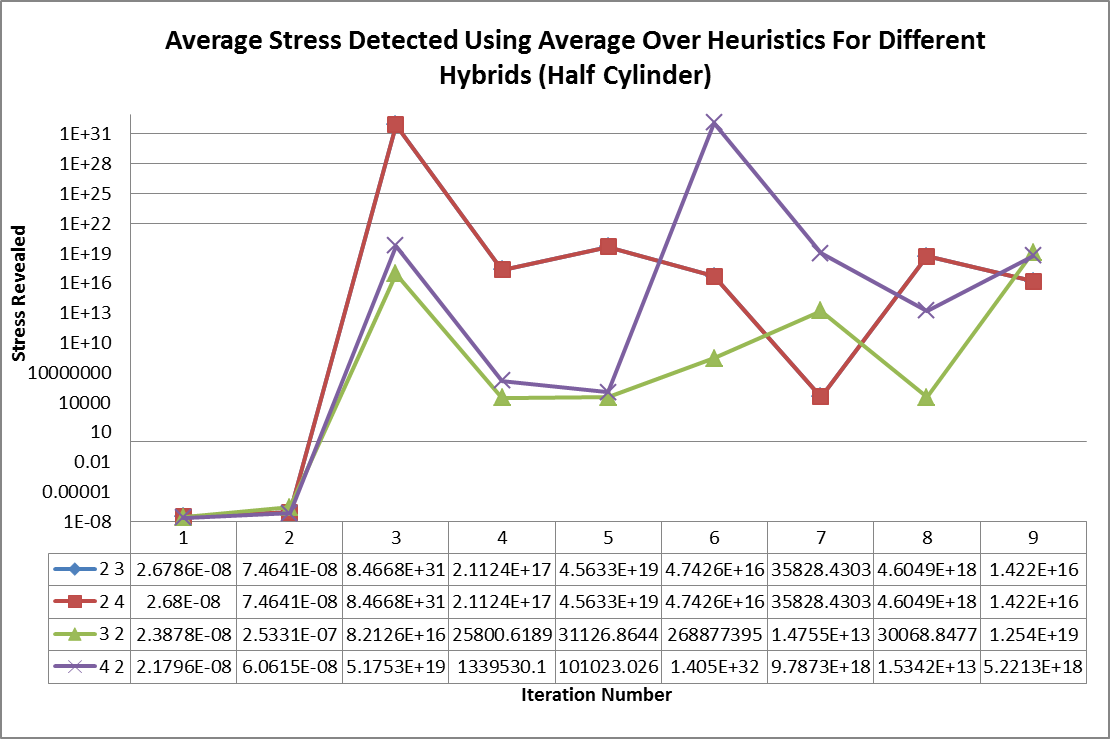
\includegraphics[width=120mm, scale=0.5]{../Graphics/HalfCylinder/AverageStressDetectedUsingAverageOverHeuristicsForDifferentHybrids(HalfCylinder).png}}
  \caption{Stress revealed for each iteration using the different hybrid methods}
\end{figure}

\begin{figure}[H]
  \centerline{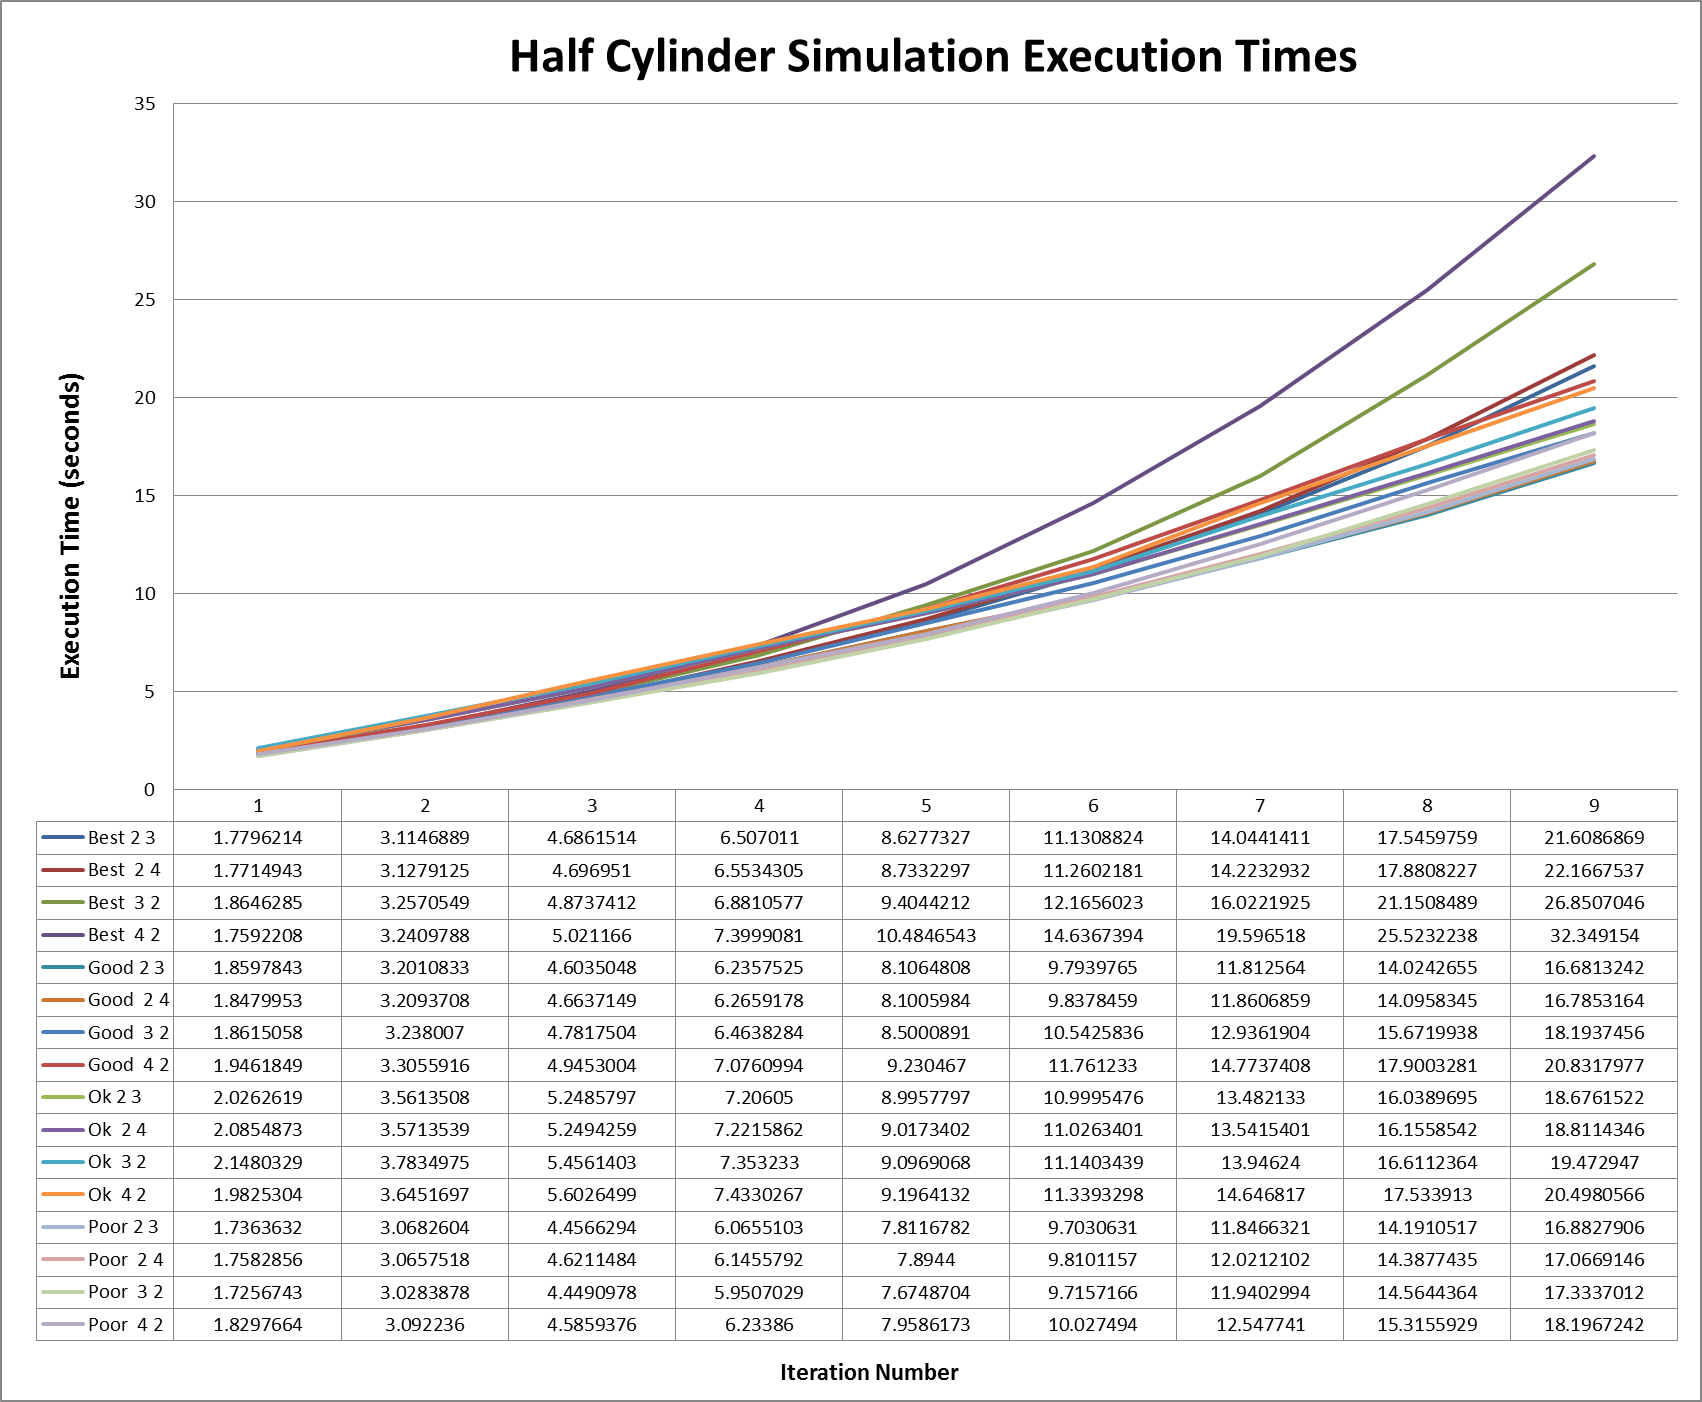
\includegraphics[width=120mm, scale=0.5]{../Graphics/HalfCylinder/ExecutionTimes.png}}
  \caption{Time taken per iteration using the different hybrid weightings with varying edge quality specifications}
\end{figure}

 
\section{Gantt Chart for Project Time Management}
\pagestyle{empty}
\begin{landscape}
\vspace*{1cm}
\hspace*{-3cm}
\begin{figure}[H]
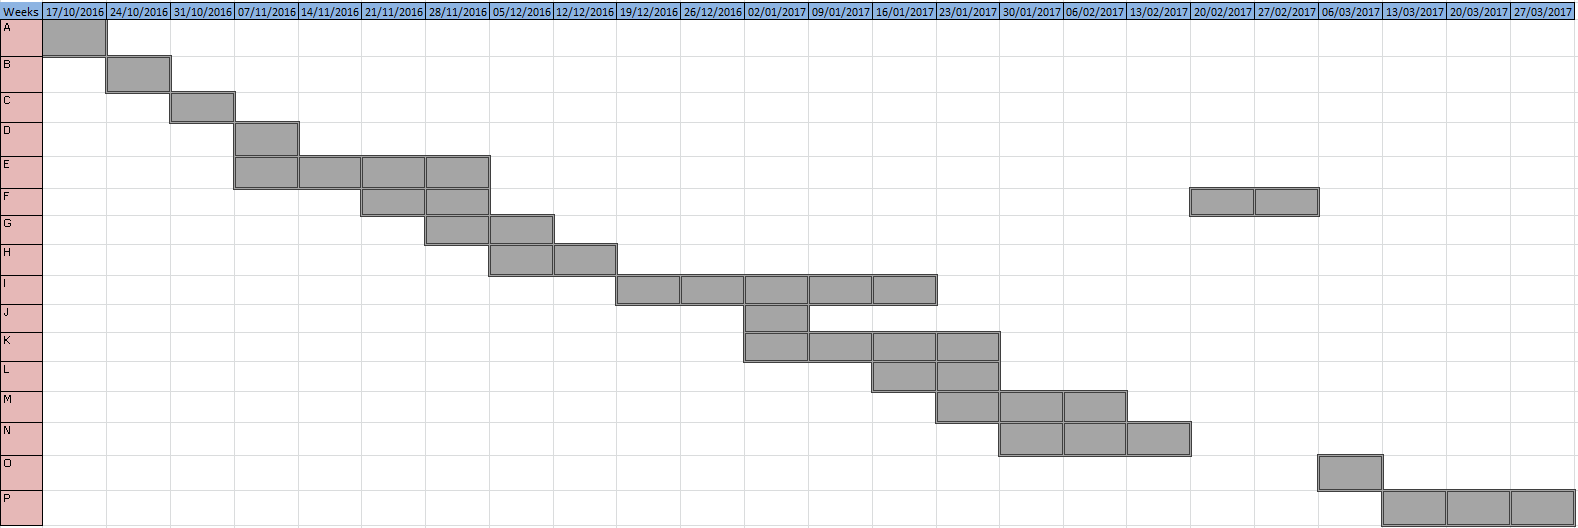
\includegraphics[width =700px, height=300px]{../Graphics/TimePlanUpdated2.png} \par
\end{figure}
\end{landscape}

